\documentclass[12pt]{article}
%\usepackage[latin1]{inputenc}
\usepackage[T1]{fontenc}
\usepackage{geometry}
\usepackage{graphicx}
\usepackage{subcaption}
\usepackage[onehalfspacing]{setspace}
\usepackage{amsmath,amsfonts,amssymb,amsthm}
\usepackage{bm}
\usepackage{commath}
\usepackage{enumerate}
\usepackage{accents}
%\usepackage{enumitem}
\usepackage[shortlabels]{enumitem}
\usepackage{dsfont}
\usepackage{mathtools}
\usepackage{physics}
\usepackage{cite}
\usepackage[round]{natbib}
\usepackage{caption}
\captionsetup[figure]{font=small}
\usepackage{float}
\usepackage{hyperref}

\newtheorem*{theorem}{Theorem} 
\newtheorem*{lemma}{Lemma}
\newtheorem*{definition}{Definition}
\newtheorem*{corollary}{Corollary}
\newtheorem*{remark}{Remark}
\newtheorem*{example}{Example}
\newtheorem*{examples}{Examples}
\newcommand*{\QEDB}{\hfill\ensuremath{\square}}

\DeclareMathOperator*{\argmax}{arg\,max}
\DeclareMathOperator*{\argmin}{arg\,min}

\newcommand\independent{\protect\mathpalette{\protect\independenT}{\perp}}
\def\independenT#1#2{\mathrel{\rlap{$#1#2$}\mkern2mu{#1#2}}}

\interfootnotelinepenalty=10000
\allowdisplaybreaks
\geometry{
  left=2.5cm,
  right=2.5cm,
  top=2cm,
  bottom=2cm,
}

\graphicspath{{C:/Users/Simon/OneDrive/Uni/LMU/SS 2020/Statistisches Consulting/Bundestag-MP-Analyse/plots/}}

\begin{document}

\section{Data}

\subsection{Data Collection}

The current political landscape of Germany consists of six parties: the right-wing \textit{AfD}, the Greens (\textit{Bündnis 90/Die Grünen}), the Christian Democrats (\textit{CDU/CSU}), the Left Party (\textit{Die Linke}), the liberal \textit{FDP}, and the Social Democrats (\textit{SPD}). These parties are represented in the German parliament (\textit{Bundestag}) according to the votes obtained during the 2017 German federal election (\textit{Bundestagswahl}), which took place on September 24, 2017. The legislative period amounts to 4 years, thus ending around September 2021. The parliament currently contains a total of 709 seats. The large majority of members of the German parliament (\textit{Abgeordnete}) are assigned a single electoral district (\textit{Wahlkreis}), the remaining ones do not have one.

In order to analyze German political entities based on text data, we constructed a broad database containing personal and Twitter data on an MP level as well as socioeconomic and election data on an electoral-district level, as detailed in the rest of this section. While parts of this database were used in the subsequent topic model analysis, it is also to be used in future text-based analyses regarding German politics. As a first step in constructing the database, we gathered personal information on all German MPs. Using Python's \textit{BeautifulSoup} web scraping tool as well as a selenium webdriver, we gathered data such as name, party, biographical information, electoral district, and social media accounts from the \href{https://www.bundestag.de/abgeordnete}{official parliament website} for all of the 709 members of the German parliament during its 19th election period, elected on September 24, 2017.\footnote{As of March 30, 2020, the official parliament website contained information on 730 MPs. This is because MPs who resigned or passed away since the beginning of the election period are also listed on the website. These MPs were manually excluded from further analysis.} An additional source of personal MP-level information would be the MPs' personal homepages. However, after inspecting some of these personal homepages at random, we found that there is no systematic way to scrape them. Furthermore, hardly any of these websites contain any informative text data comparable to tweets or Facebook posts. As a consequence, we decided against further pursuing this potential source of information. Due to difficulties and recent restrictions when scraping Facebook data, caused in parts by the aforementioned data scandal, we also discarded Facebook as source of text data and focused solely on Twitter. 

Since information on social media profiles was scarce and incomplete on the official parliament website, we additionally scraped official party homepages of all of the six political parties represented in the current parliament.\footnote{The official homepage of the AfD party does not provide the Twitter profiles of their members, which is why for this party we had to manually gather the account names.} MPs who did not provide a Twitter account either on the official parliament website or on their party's official homepage were excluded. Using Python's \textit{tweepy} library to access the official Twitter API, we scraped all tweets by German MPs from September 24, 2017 through April 24, 2020, i.e., during a total of 31 months. The \textit{tweepy} library offers a variety of additional features to be extracted apart from the mere tweet texts, such as the number of followers of an account, retweets, or how many times a tweet was like or retweeted. While we only use original tweets in the analysis presented in this paper, we included the most relevant additional Twitter features in our database, for use in future analyses. This initially yielded 342,542 tweets from a total of 470 members of parliament.\footnote{\textit{tweepy} restricts the total number of tweets retrievable to 3,200. For those MPs who tweeted more than 3,200 tweets during our period of analysis, the most recent 3,200 tweets were taken into account. However, this only applied to two MPs.}

To complement personal and Twitter data, we also gathered socioeconomic data such as GDP per capita and unemployment rate as well as 2017 election results on an electoral-district level for all of the 299 electoral districts from the \href{https://www.bundeswahlleiter.de}{official electoral website}. After removing the only MP labeled as independent (\textit{fraktionslos}) on the official electoral website as well as 19 MPs without a specific electoral district assigned to them (for matchability with socioeconomic data), the final dataset counted 450 MPs. Overall, 63\% of all 709 MPs were thus included in the analysis. The corresponding total number of tweets amounted to 323,740. For those MPs without elecotoral district, electoral district-level socioeconomic variables could potentially be imputed by using state averages or values of nearby and/or similar districts. However, given that this only applies to 19 out of the remaining 450 MPs and since imputing covariates would introduce further uncertainty, we decided to exclude those MPs.

The table below shows total monthly tweet frequencies for our period of analysis, September 24, 2017 through April 24, 2020. As can be seen, tweet frequencies - though fluctuating - show an increasing trend over time, peaking at almost 20,000 in March 2020. The decrease for April 2020 can partly be explained by the fact that only the first 24 days of the month were taken into account.

\begin{figure}[h!]
  \centering
  \captionsetup{justification=centering,margin=2cm}
  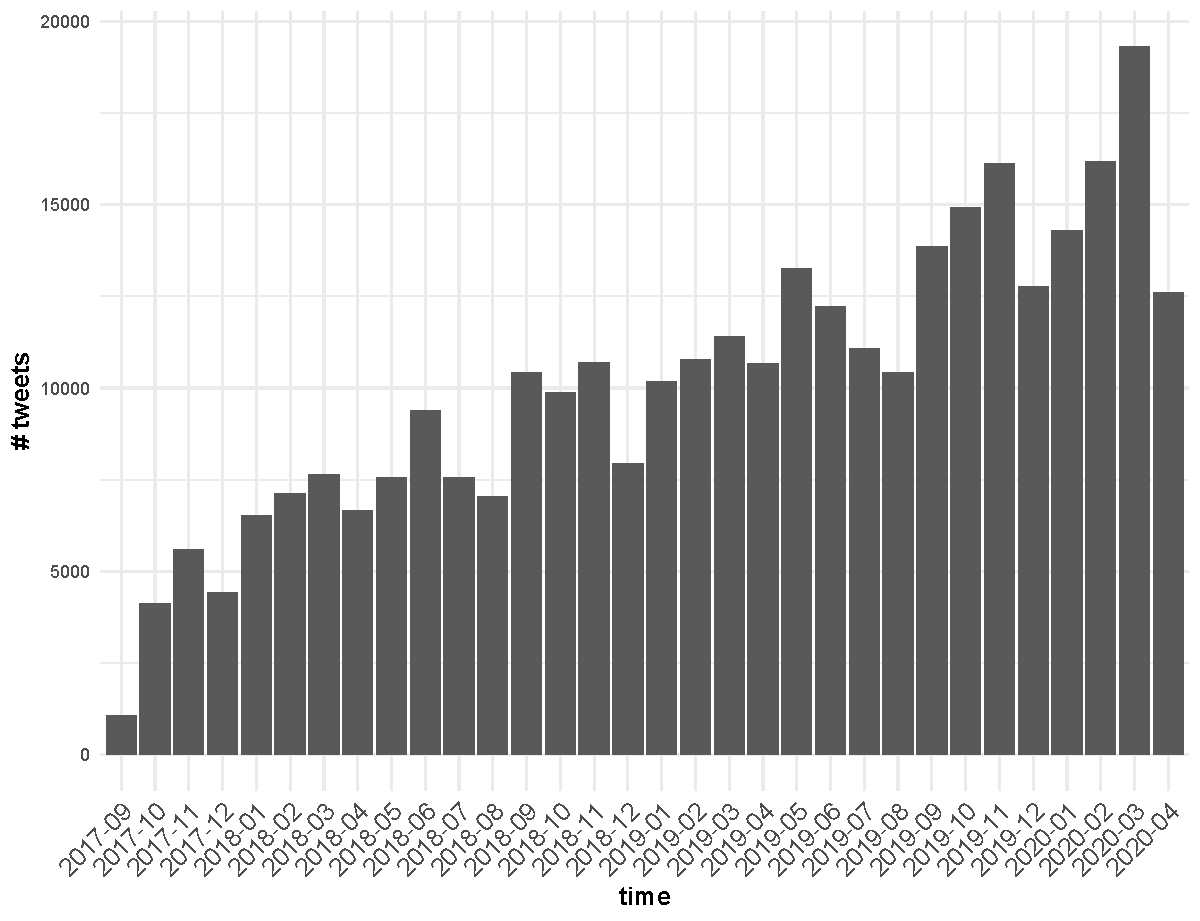
\includegraphics[scale = 0.5]{3/monthly_tweets.pdf}
  \caption{Monthly tweet volume by German MPs from September 24, 2017 through April 24, 2020.}
  \label{fig:monthly_tweets}
\end{figure}

Next, data was grouped and tweets were concatenated on a per-user level (thus aggregating tweets across the entire 31 months) as well as on a per-user per-month level, yielding a user-level and a monthly dataset. This means that a document represents the concatenation of \textit{all} of a single MP's tweets for the user-level dataset, while it represents a single MP's \textit{monthly} tweets for the monthly dataset. This also means that MP-level metadata such as personal information and socioeconomic data (through the electoral-district matching) can be used as document-level covariates. For the monthly dataset, the temporal component (year and month) constitutes an additional covariate. Since it is reasonable to assume that the importance of topics varies over time and due to resulting documents being shorter and more easily interpretable, we chose the monthly dataset for further analysis.\footnote{For instance, as stated in section 4.2, one topic is about COVID-19, which is clearly a relatively recent topic. The monthly dataset allows for tracing the development of this topic's relevance over time: a flat curve until January 2020, followed by a sharp increase during the first months of 2020. The user-level dataset, on the other hand, would simply assign a low overall proportion to this topic.} At this point, the data preparation was completed, marking the starting point of the preprocessing required for topic analysis, which is identical for both the user-level and the monthly dataset.

\subsection{Data Preprocessing}

We used the \textit{quanteda} package within the R programming language for preprocessing. As a first step, we built a quanteda corpus from all documents. Next, we immediately transcribed German umlauts \textit{ä/Ä}, \textit{ö/Ö}, \textit{ü/Ü} as well as German ligature \textit{ß} as \textit{ae/Ae}, \textit{oe/Oe}, \textit{ue/Ue}, and \textit{ss}, respectively, and removed hyphens. Subsequently, we transformed the text data into a quanteda document-feature matrix (DFM), which essentially tokenizes texts, thereby converting all characters to lowercase. From the DFM, we removed an extensive list of German stopwords, using the \href{https://github.com/stopwords-iso/stopwords-iso}{stopwords-iso GitHub repository}, as well as English stopwords included in the \textit{quanteda} package. Moreover, hashtags, usernames, quantities and units (e.g., \textit{10kg} or \textit{14.15uhr}), interjections (e.g., \textit{aaahhh} or \textit{ufff}), terms containing non-alphanumerical characters, meaningless word stumps (e.g., \textit{innen} from the German female plural declension, or \textit{amp}, the remainder left after removing the ampersand sign, \textit{\&}) were removed. Terms with less than four characters and terms with a term frequency (overall number of occurrences) below five or with a document frequency (number of documents containing the word) below three were excluded. Finally, we manually removed overly frequent terms that would diminish the distinguishability of topics, such as \textit{bundestag} or \textit{polit} (see \textit{semantic coherence} in section 4.1 for a technical explanation).

We also performed word-stemming, which means cutting off word endings to remove discrepancies arising purely from declensions or conjugations, being of particular importance for the German language. Due to the nature of the German language, the additional gains of lemmatization (which aims at identifying the base form of each word) would only be small as compared to the large increase in complexity, which is why we decided to use stemming only. Another issue when dealing with German language documents is represented by compound words, which are sometimes hyphenated, basically leading to a distinction where semantically there is none. We addressed this issue by removing hyphens in the very beginning of the preprocessing and converting all terms to lowercase, thus "gluing together" compound words; this way, terms like \textit{Bundesregierung} and \textit{Bundes-Regierung} are both transformed into \textit{bundesregierung} (and, after stemming, into \textit{bundesregier}). Finally, automatic segmentation techniques were not necesssary for the German language (\citealp{lucas2015computer}). As a result of preprocessing, one empty MP-level document was dropped, so that a total of 10,998 (monthly) MP-level documents were eventually analyzed, each one associated with 90 covariates.


\bibliography{bibliography}
\bibliographystyle{plainnat}

\end{document}